\documentclass[tikz,border=15pt]{standalone}
\usepackage{amsmath,amssymb}
\usetikzlibrary{calc}

\begin{document}
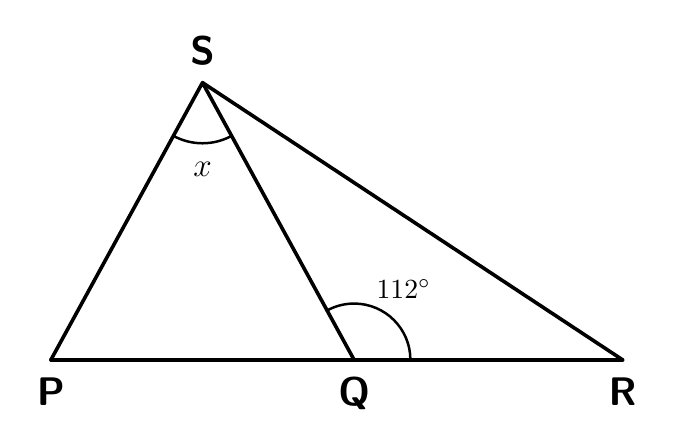
\begin{tikzpicture}[scale=1.1, line cap=round, line join=round]
  % Coordinates
  \coordinate (P) at (0, 0);
  \coordinate (Q) at (3.5, 0);
  \coordinate (R) at (6.6, 0);
  \coordinate (S) at (1.75, 3.2);

  % Triangle & collinear baseline
  \draw[line width=1.3pt] (P) -- (R);
  \draw[line width=1.3pt] (P) -- (S) -- (Q);
  \draw[line width=1.3pt] (S) -- (R);

  % Vertex labels
  \node[below=3pt, font=\Large\sffamily\bfseries] at (P) {P};
  \node[below=3pt, font=\Large\sffamily\bfseries] at (Q) {Q};
  \node[below=3pt, font=\Large\sffamily\bfseries] at (R) {R};
  \node[above=3pt, font=\Large\sffamily\bfseries] at (S) {S};

  % Angle x at S
  % S to P angle is approx 241 deg, S to Q angle is approx 299 deg
  \draw[line width=0.9pt] ($(S) + (241:0.7)$) arc (241:299:0.7);
  \node[font=\large] at ($(S) + (270:1.0)$) {$x$};

  % Exterior angle 112 at Q (from 0 to 119 deg)
  \draw[line width=0.9pt] ($(Q) + (0:0.65)$) arc (0:119:0.65);
  \node[font=\normalsize] at ($(Q) + (55:1.0)$) {$112^\circ$};

\end{tikzpicture}
\end{document}
